
%!TEX root = handout.tex

\newpage
\section{Isobaric analysis}
In the last chapters, we identified and quantified peptides in a label-free experiment. In this section, we would like to introduce a possible workflow for the analysis of isobaric data.

\subsection{Isobaric analysis workflow}
Let's have a look at the workflow (see Fig \ref{fig:isobaric_wf})

\begin{figure}[htbp]
  \centering
  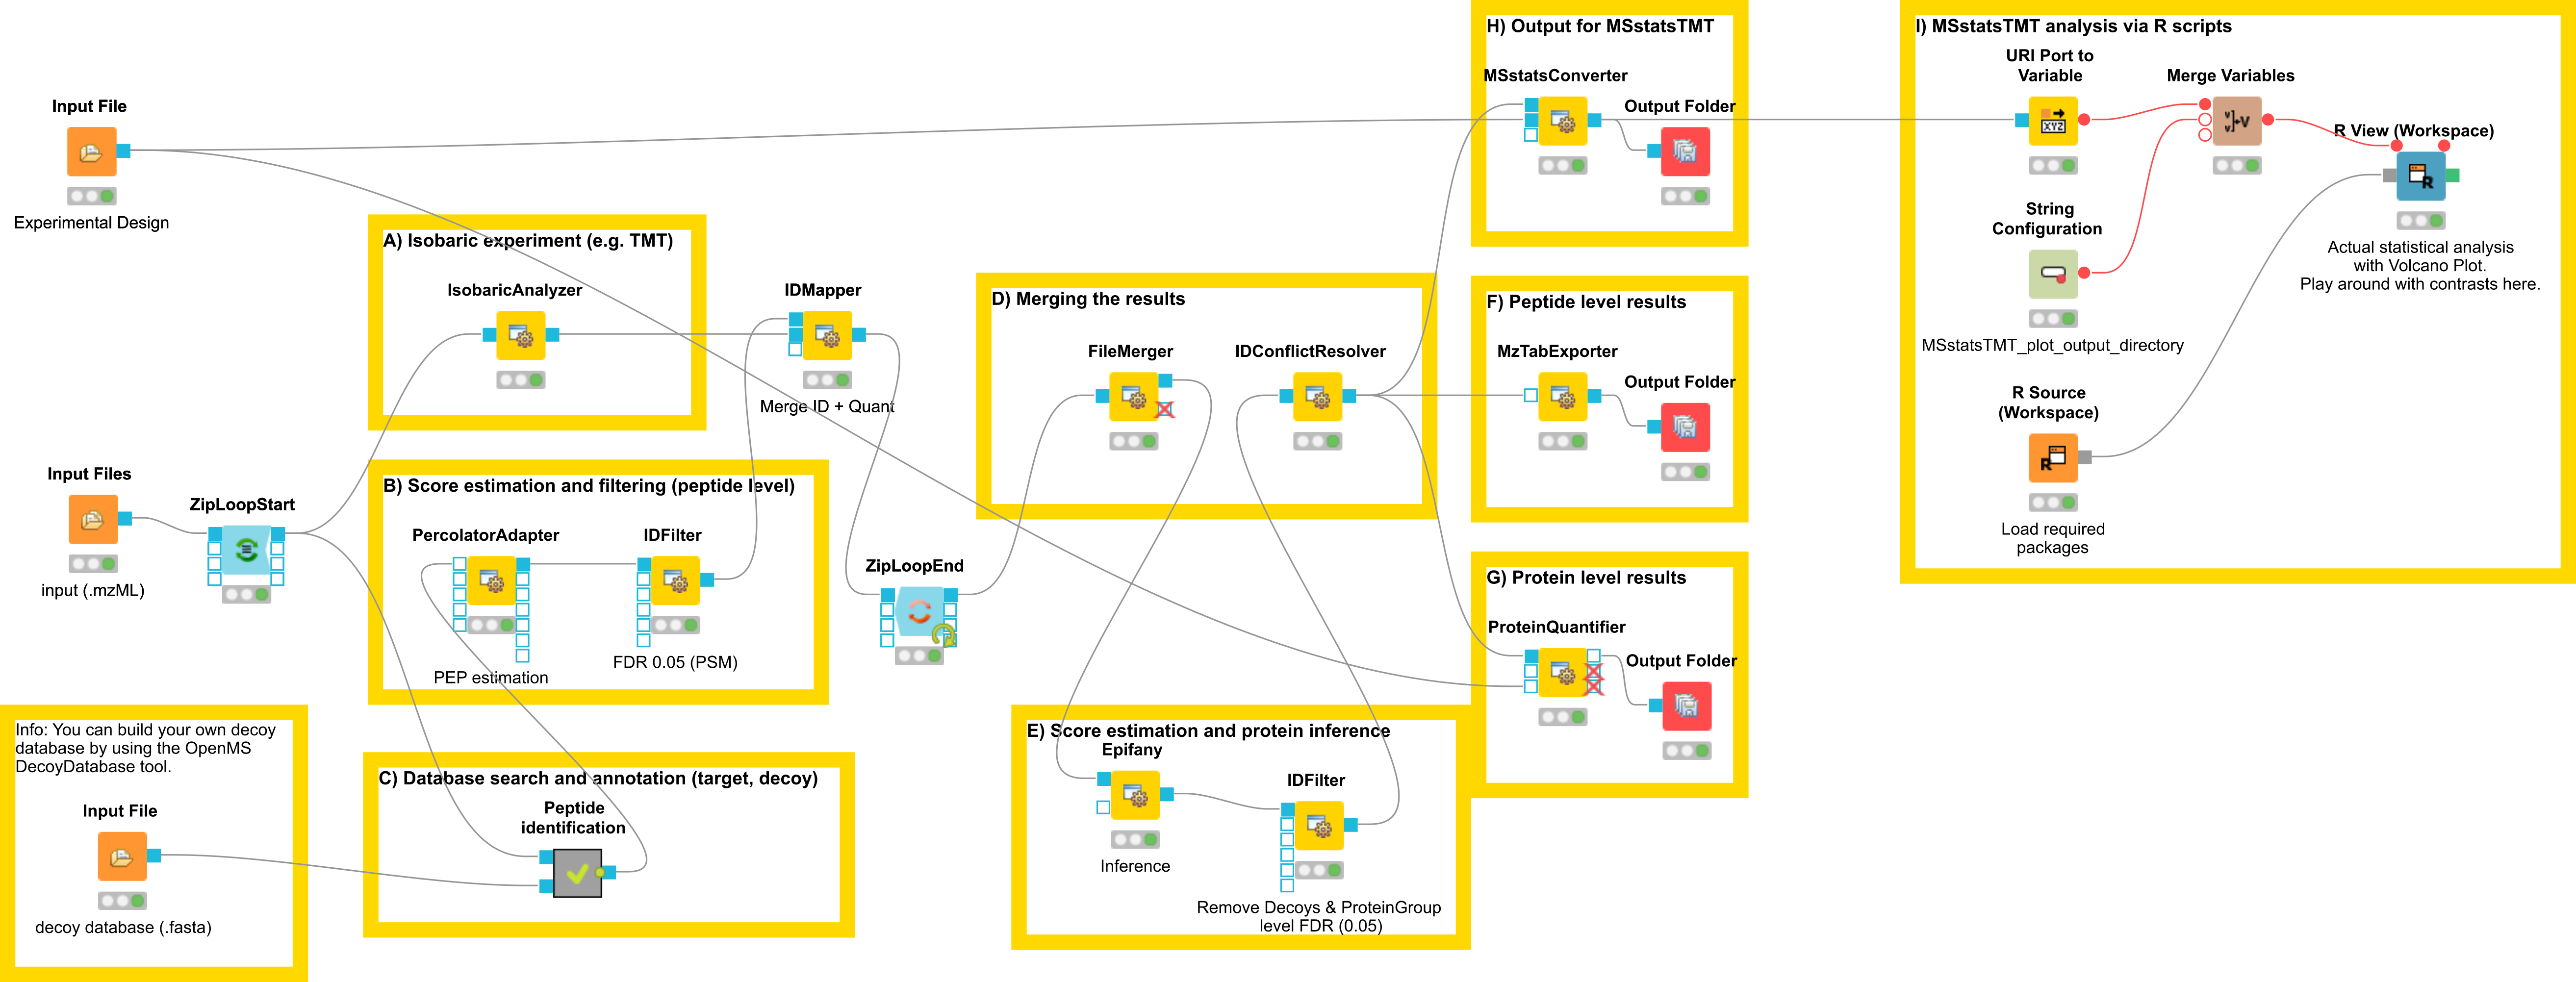
\includegraphics[width=0.95\textwidth]{graphics/isobaric/isobaric_inference_wf.png}
  \caption{Workflow for the analysis of isobaric data}
  \label{fig:isobaric_wf}
\end{figure}

\noindent The full analysis workflow can be found here: \\
\directory{Workflows/ \\ Identification\_quantification\_isobaric\_inference\_epifany\_MSstatsTMT}. \\

\noindent The workflow has four input nodes. The first for the experimental design to allow for MSstatsTMT compatible export (\KNIMENODE{MSstatsConverter}). The second for the .mzML files with the centroided spectra from the isobaric labeling experiment and the third one for the .fasta database used for identification. The last one allows to specify an output path for the plots generated by the \KNIMENODE{R View}, which runs MSstatsTMT (I). The quantification (A) is performed using the \KNIMENODE{IsobaricAnalzyer}. The tool is able to extract and normalize quantitative information from TMT and iTRAQ data. The values can be assessed from centroided MS2 or MS3 spectra (if available). Isotope correction is performed based on the specified correction matrix (as provided by the manufacturer). The identification (C) is applied as known from the previous chapters by using database search and a target-decoy database.

\noindent To reduce the complexity of the data for later inference the q-value estimation and FDR filtering is performed on PSM level for each file individually (B). Afterwards the identification (PSM) and quantiative information is combined using the \KNIMENODE{IDMapper}. After the processing of all available files, the intermediate results are aggregated (\KNIMENODE{FileMerger} - D). All PSM results are used for score estimation and protein inference (\KNIMENODE{Epifany}) (E). For detailed information about protein inference please see Chaper \ref{topic:protein_inference}. Then, decoys are removed and the inference results are filtered via a protein group FDR. Peptide level results can be exported via \KNIMENODE{MzTabExporter} (F), protein level results can be obtained via the \KNIMENODE{ProteinQuantifier} (G) or the results can exported (\KNIMENODE{MSstatsConverter} - H) and further processed with the following R pipeline to allow for downstream processing using MSstatsTMT. \\

\noindent Please import the workflow from \directory{Workflows > \\ Identification\_quantification\_isobaric\_inference\_epifany\_MSstatsTMT} into KNIME via the menu entry \menu{File > Import KNIME workflow > Select file} and double-click the imported workflow in order to open it. Before you can execute the workflow, you have to correct the locations of the files in the \KNIMENODE{Input Files} nodes (don't forget the one for the FASTA database inside the ``ID'' meta node). Try and run your workflow by executing all nodes at once.

\subsection{Excursion MSstatsTMT}
The R package MSstatsTMT can be used for protein significance analysis in shotgun mass spectrometry-based proteomic experiments with tandem mass tag (TMT) labeling. MSstatsTMT provides functionality for two types of analysis \& their visualization: Protein summarization based on peptide quantification and Model-based group comparison to detect significant changes in abundance. It depends on accurate feature detection, identification and quantification which can be performed e.g. by an OpenMS workflow. \\

\noindent In general MSstatsTMT can be used for data processing \& visualization, as well as statistical modeling. Please see ~\cite{Huang2020} and \url{http://msstats.org/msstatstmt/} for further information. \\

\noindent There is also a very helpful online lecture and tutorial for MSstatsTMT from the May Institute Workshop 2020. Please see \url{https://youtu.be/3CDnrQxGLbA}

\subsection{Dataset \& Experimental Design}
We are using the MSV000084264 ground truth dataset, which consits of TMT10plex controlled mixes of different concentrated UPS1 peptides spiked into SILAC HeLa peptides measured in a dilution series \url{https://www.omicsdi.org/dataset/massive/MSV000084264}. Figure \ref{fig:isobaric_experimental_design} shows the experimental design. In this experiment 5 different TMT10plex mixtures -- different labeling strategies -- were analysed. These were measured in triplicates represented by the 15 MS runs (3 runs each). 

\begin{figure}[htbp]
  \centering
 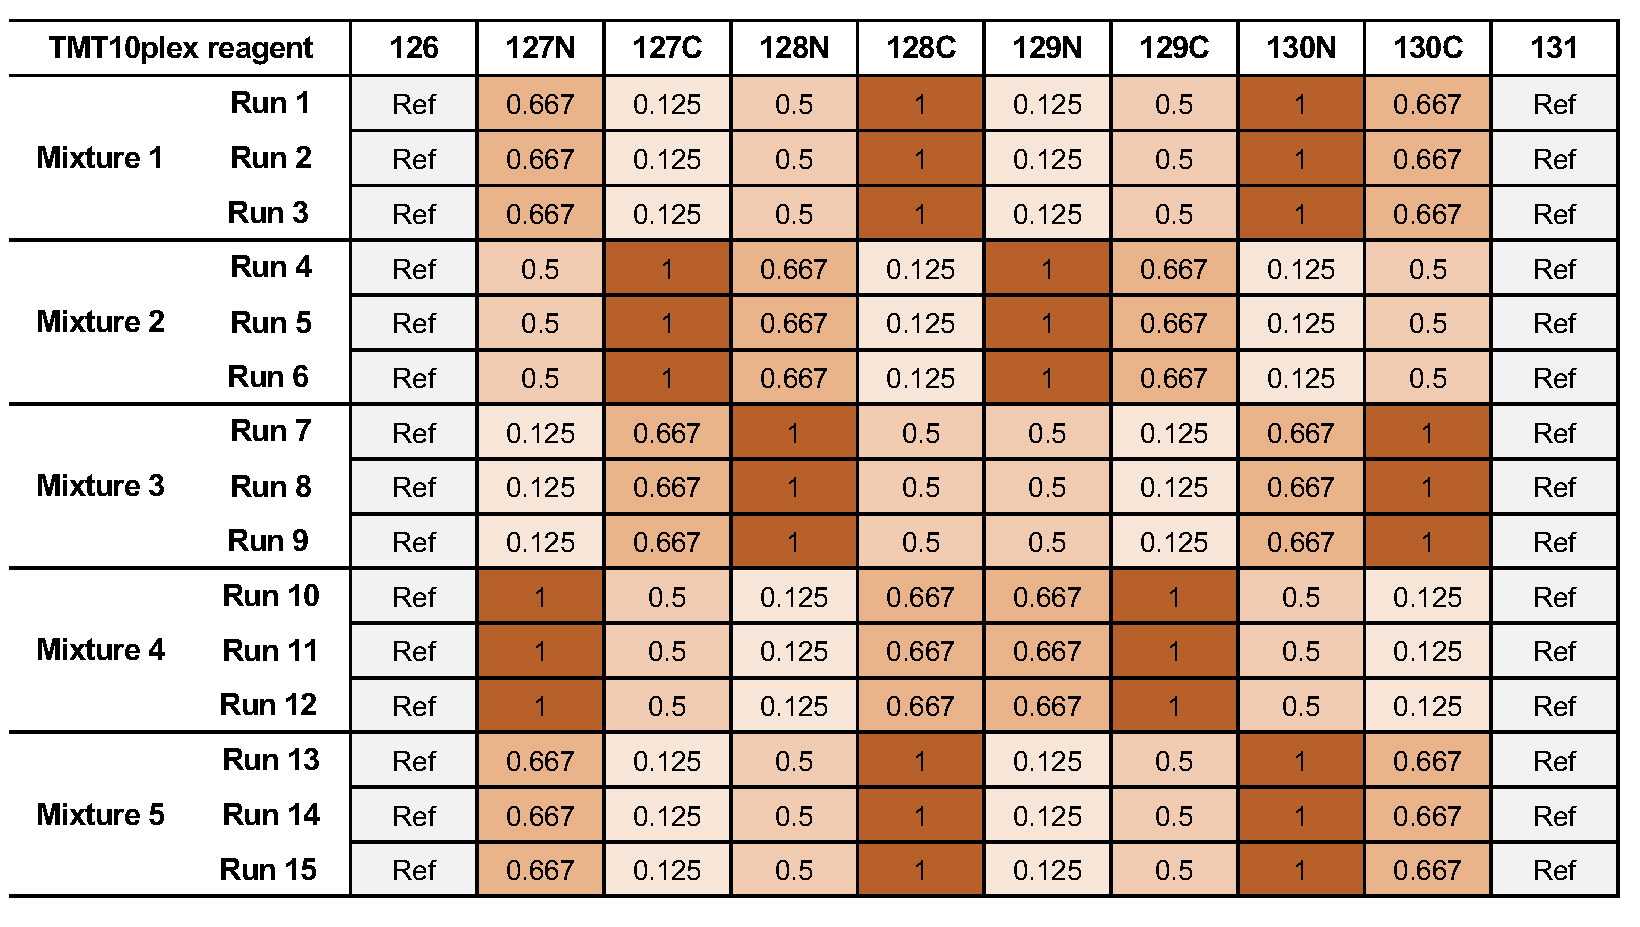
\includegraphics[width=0.95\textwidth]{graphics/isobaric/isobaric_experimental_design.jpg}
  \caption{Experimental Design}
  \label{fig:isobaric_experimental_design}
\end{figure}
  
\noindent The experimental design in table format allows for MSstatsTMT compatible export. The design is represented by two tables. The first one \ref{t:isobaric_experimental_design_table_0} represents the overall structure of the experiment in terms of samples, fractions, labels and fraction groups. The second one \ref{t:isobaric_experimental_design_table_1} adds to the first by specifying specific conditions, biological replicates as well as mixtures and label for each channel. For additional information about the experimental design please see Table  \ref{t:Experimental_design_exp} in Chapter \ref{topic:experimental_design}. 

\begin{table}[ht]
\caption{Experimental Design 1}
\label{t:isobaric_experimental_design_table_0}
\centering
\tiny
\begin{tabular*}{0.90\textwidth}{lllll}
Spectra\_Filepath & Fraction & Label & Fraction\_Group & Sample \\
161117\_SILAC\_HeLa\_UPS1\_TMT10\_SPS\_MS3\_Mixture1\_01.mzML & 1        & 1     & 1               & 1      \\
161117\_SILAC\_HeLa\_UPS1\_TMT10\_SPS\_MS3\_Mixture1\_01.mzML & 1        & 2     & 1               & 2      \\
161117\_SILAC\_HeLa\_UPS1\_TMT10\_SPS\_MS3\_Mixture1\_01.mzML & 1        & 3     & 1               & 3      \\
161117\_SILAC\_HeLa\_UPS1\_TMT10\_SPS\_MS3\_Mixture1\_01.mzML & 1        & 4     & 1               & 4      \\
161117\_SILAC\_HeLa\_UPS1\_TMT10\_SPS\_MS3\_Mixture1\_01.mzML & 1        & 5     & 1               & 5      \\
161117\_SILAC\_HeLa\_UPS1\_TMT10\_SPS\_MS3\_Mixture1\_01.mzML & 1        & 6     & 1               & 6      \\
161117\_SILAC\_HeLa\_UPS1\_TMT10\_SPS\_MS3\_Mixture1\_01.mzML & 1        & 7     & 1               & 7      \\
161117\_SILAC\_HeLa\_UPS1\_TMT10\_SPS\_MS3\_Mixture1\_01.mzML & 1        & 8     & 1               & 8      \\
161117\_SILAC\_HeLa\_UPS1\_TMT10\_SPS\_MS3\_Mixture1\_01.mzML & 1        & 9     & 1               & 9      \\
161117\_SILAC\_HeLa\_UPS1\_TMT10\_SPS\_MS3\_Mixture1\_01.mzML & 1        & 10   & 1               & 10     \\
161117\_SILAC\_HeLa\_UPS1\_TMT10\_SPS\_MS3\_Mixture1\_02.mzML & 1        & 1     & 2               & 11     \\
161117\_SILAC\_HeLa\_UPS1\_TMT10\_SPS\_MS3\_Mixture1\_02.mzML & 1        & 2     & 2               & 12     \\
161117\_SILAC\_HeLa\_UPS1\_TMT10\_SPS\_MS3\_Mixture1\_02.mzML & 1        & 3     & 2               & 13     \\
161117\_SILAC\_HeLa\_UPS1\_TMT10\_SPS\_MS3\_Mixture1\_02.mzML & 1        & 4     & 2               & 14     \\
161117\_SILAC\_HeLa\_UPS1\_TMT10\_SPS\_MS3\_Mixture1\_02.mzML & 1        & 5     & 2               & 15     \\
161117\_SILAC\_HeLa\_UPS1\_TMT10\_SPS\_MS3\_Mixture1\_02.mzML & 1        & 6     & 2               & 16     \\
161117\_SILAC\_HeLa\_UPS1\_TMT10\_SPS\_MS3\_Mixture1\_02.mzML & 1        & 7     & 2               & 17     \\
161117\_SILAC\_HeLa\_UPS1\_TMT10\_SPS\_MS3\_Mixture1\_02.mzML & 1        & 8     & 2               & 18     \\
161117\_SILAC\_HeLa\_UPS1\_TMT10\_SPS\_MS3\_Mixture1\_02.mzML & 1        & 9     & 2               & 19     \\
161117\_SILAC\_HeLa\_UPS1\_TMT10\_SPS\_MS3\_Mixture1\_02.mzML & 1        & 10   & 2               & 20     \\
161117\_SILAC\_HeLa\_UPS1\_TMT10\_SPS\_MS3\_Mixture1\_03.mzML & 1        & 1     & 3               & 21     \\
161117\_SILAC\_HeLa\_UPS1\_TMT10\_SPS\_MS3\_Mixture1\_03.mzML & 1        & 2     & 3               & 22     \\
161117\_SILAC\_HeLa\_UPS1\_TMT10\_SPS\_MS3\_Mixture1\_03.mzML & 1        & 3     & 3               & 23     \\
161117\_SILAC\_HeLa\_UPS1\_TMT10\_SPS\_MS3\_Mixture1\_03.mzML & 1        & 4     & 3               & 24     \\
161117\_SILAC\_HeLa\_UPS1\_TMT10\_SPS\_MS3\_Mixture1\_03.mzML & 1        & 5     & 3               & 25     \\
161117\_SILAC\_HeLa\_UPS1\_TMT10\_SPS\_MS3\_Mixture1\_03.mzML & 1        & 6     & 3               & 26     \\
161117\_SILAC\_HeLa\_UPS1\_TMT10\_SPS\_MS3\_Mixture1\_03.mzML & 1        & 7     & 3               & 27     \\
161117\_SILAC\_HeLa\_UPS1\_TMT10\_SPS\_MS3\_Mixture1\_03.mzML & 1        & 8     & 3               & 28     \\
161117\_SILAC\_HeLa\_UPS1\_TMT10\_SPS\_MS3\_Mixture1\_03.mzML & 1        & 9     & 3               & 29     \\
161117\_SILAC\_HeLa\_UPS1\_TMT10\_SPS\_MS3\_Mixture1\_03.mzML & 1        & 10   & 3               & 30    
\end{tabular*}
\end{table}
  
\begin{table}[ht]
\caption{Experimental Design 2}
\label{t:isobaric_experimental_design_table_1}
\centering
\tiny
\begin{tabular*}{0.90\textwidth}{lllll}
Sample & MSstats\_Condition & MSstats\_BioReplicate & MSstats\_Mixture & LabelName \\
1      & Norm               & Norm                  & 1                & 126       \\
2      & 0.667              & 0.667                 & 1                & 127N      \\
3      & 0.125              & 0.125                 & 1                & 127C      \\
4      & 0.5                & 0.5                   & 1                & 128N      \\
5      & 1                  & 1                     & 1                & 128C      \\
6      & 0.125              & 0.125                 & 1                & 129N      \\
7      & 0.5                & 0.5                   & 1                & 129C      \\
8      & 1                  & 1                     & 1                & 130N      \\
9      & 0.667              & 0.667                 & 1                & 130C      \\
10     & Norm               & Norm                  & 1                & 131       \\
11     & Norm               & Norm                  & 1                & 126       \\
12     & 0.667              & 0.667                 & 1                & 127N      \\
13     & 0.125              & 0.125                 & 1                & 127C      \\
14     & 0.5                & 0.5                   & 1                & 128N      \\
15     & 1                  & 1                     & 1                & 128C      \\
16     & 0.125              & 0.125                 & 1                & 129N      \\
17     & 0.5                & 0.5                   & 1                & 129C      \\
18     & 1                  & 1                     & 1                & 130N      \\
19     & 0.667              & 0.667                 & 1                & 130C      \\
20     & Norm               & Norm                  & 1                & 131       \\
21     & Norm               & Norm                  & 1                & 126       \\
22     & 0.667              & 0.667                 & 1                & 127N      \\
23     & 0.125              & 0.125                 & 1                & 127C      \\
24     & 0.5                & 0.5                   & 1                & 128N      \\
25     & 1                  & 1                     & 1                & 128C      \\
26     & 0.125              & 0.125                 & 1                & 129N      \\
27     & 0.5                & 0.5                   & 1                & 129C      \\
28     & 1                  & 1                     & 1                & 130N      \\
29     & 0.667              & 0.667                 & 1                & 130C      \\
30     & Norm               & Norm                  & 1                & 131   
\end{tabular*}
\end{table}

\noindent After running the worklfow the \KNIMENODE{MSstatsConverter} will convert the OpenMS output in addition with the experimental design to a file (.csv) which can be processed by using MSstatsTMT.

\subsubsection{MSstatsTMT analysis}
Here, we depict the analysis by MSstatsTMT using a segment of the isobaric analysis workflow (Fig. \ref{fig:isobaric_msstatstmtwf} ). The segment is available as \directory{Workflows/ MSstatsTMT.knwf}. \\

\begin{figure}[htbp]
\caption{MSstatsTMT workflow segment}
\centering
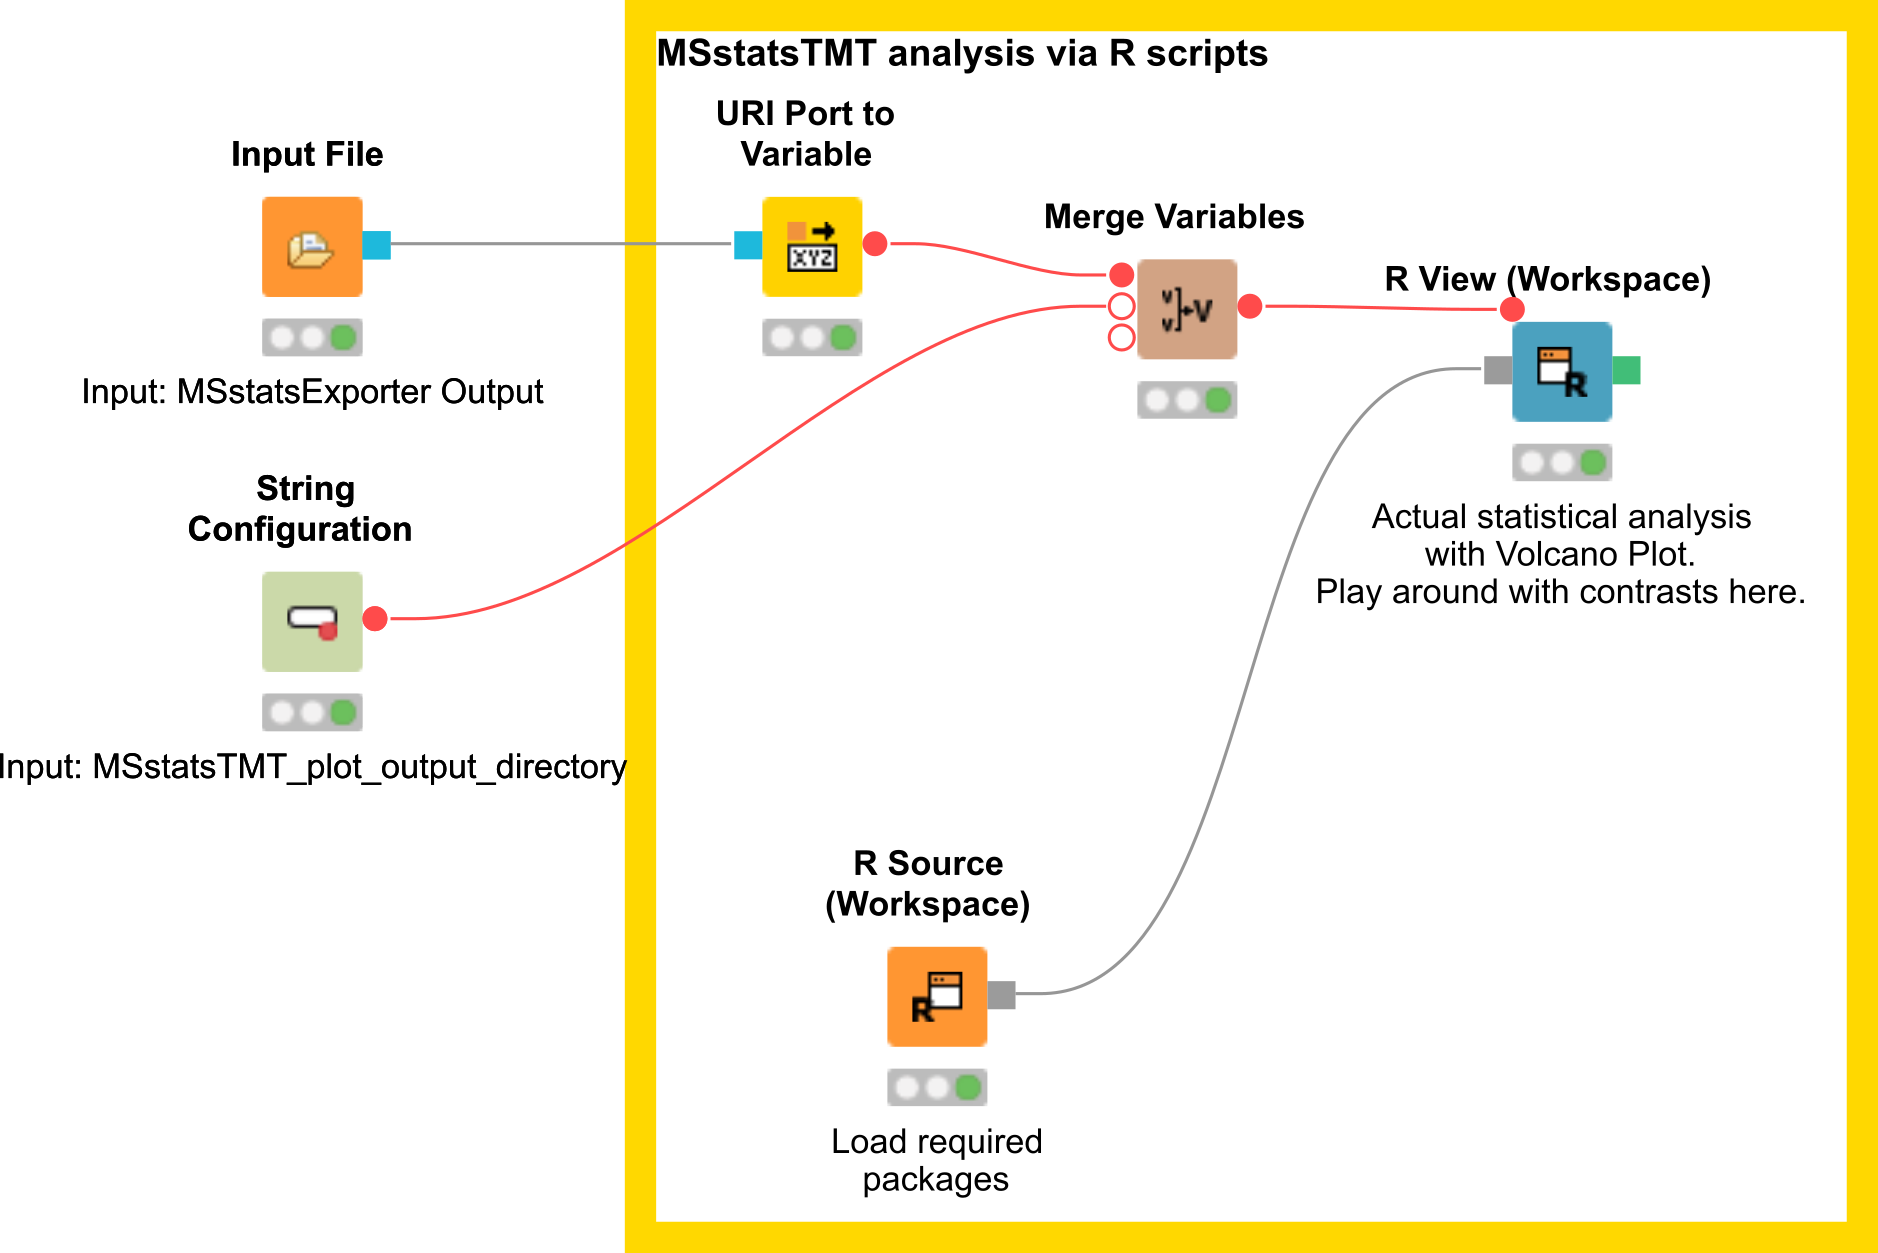
\includegraphics[width=0.80\textwidth]{graphics/isobaric/isobaric_msstatstmt_wf.png}
 \label{fig:isobaric_msstatstmtwf}
\end{figure}

\noindent There are two input nodes, the first one takes the result (.csv) from the \KNIMENODE{MSstatsConverter} and the second a path to the directory where the plots generated by MSstatsTMT should be saved. The \KNIMENODE{R source} node loads the required packages, such as dplyr for data wrangling, MSstatsTMT for analysis and MSstats for plotting. The inputs are further processed in the \KNIMENODE{R View} node.  

\noindent Here, the data of the \KNIMENODE{Input File} is loaded into R using the flow variable ["URI-0"]:
\begin{lstlisting}
file <- substr(knime.flow.in[["URI-0"]], 6, nchar(knime.flow.in[["URI-0"]]))
MSstatsConverter_OpenMS_out <- read.csv(file)
data <- MSstatsConverter_OpenMS_out
\end{lstlisting}

\noindent The OpenMStoMSstatsTMTFormat function preprocesses the OpenMS report and converts it into the required input format for MSstatsTMT, by filtering based on unique peptides and measurments in each MS run.

\begin{lstlisting}
processed.data <- OpenMStoMSstatsTMTFormat(data)
\end{lstlisting}

\noindent Afterwards different normalization steps are performed (global, protein, runs) as well as data imputation by using the msstats method. In addition peptide level data is summarized to protein level data. 

\begin{lstlisting}
quant.data <- proteinSummarization(processed.data,
                                   method="msstats",
                                   global_norm=TRUE,
                                   reference_norm=TRUE,
                                   MBimpute = TRUE,
                                   maxQuantileforCensored = NULL,
                                   remove_norm_channel = TRUE,
                                   remove_empty_channel =  TRUE)
\end{lstlisting}
        
\noindent There a lot of different possibilities to configure this method please have a look at the MSstatsTMT package for additional detailed information \url{http://bioconductor.org/packages/release/bioc/html/MSstatsTMT.html}                       

\noindent The next step is the comparions of the different conditions, here either a pairwise comparision can be performed or a confusion matrix can be created. The goal is to detect and compare the UPS peptides spiked in at different concentrations. 

\begin{lstlisting}
# prepare contrast matrix
unique(quant.data$Condition)

comparison<-matrix(c(-1,0,0,1,
                     0,-1,0,1,
                     0,0,-1,1,
                     0,1,-1,0,
                     1,-1,0,0), nrow=5, byrow = T)
                     
# Set the names of each row
row.names(comparison)<- contrasts <- c("1-0125",   
                                       "1-05",  
                                       "1-0667",
                                       "05-0667",
                                       "0125-05")
# Set the column names
colnames(comparison)<- c("0.125", "0.5", "0.667", "1")

\end{lstlisting}

\noindent The constructed confusion matrix is used in the groupComparisonTMT function to test for significant changes in protein abundance across conditions based on a family of linear mixed-effects models in TMT experiments. 

\begin{lstlisting}
data.res <- groupComparisonTMT(data = quant.data, 
                               contrast.matrix = comparison,
                               moderated = TRUE, # do moderated t test
                               adj.method = "BH") # multiple comparison adjustment
data.res <- data.res %>% filter(!is.na(Protein))
\end{lstlisting}

\noindent  In the next step the comparison can be plotted using the groupComparisonPlots function by MSstats

\begin{lstlisting}
library(MSstats)
groupComparisonPlots(data=data.res.mod, type="VolcanoPlot", address=F, which.Comparison = "0125-05", sig = 0.05)
\end{lstlisting}

\noindent  Here, we have a example output of the \KNIMENODE{R View}, which depicts the significant regulated  UPS proteins in the comparison of 125 to 05 (Fig. \ref{fig:isobaric_volcanoplot}). 

\begin{figure}[htbp]
  \centering
 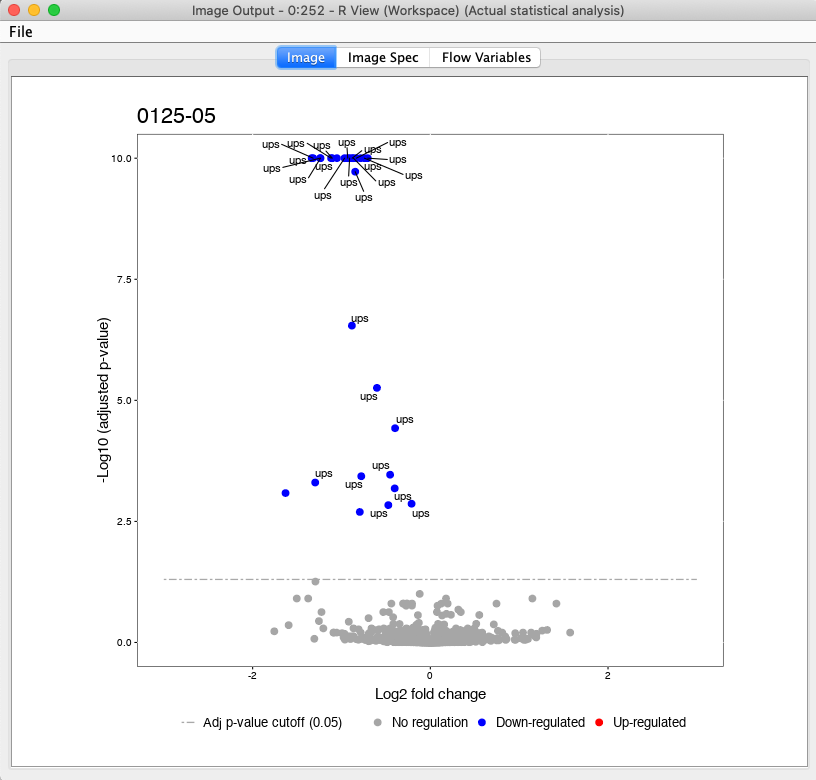
\includegraphics[width=0.80\textwidth]{graphics/isobaric/isobaric_img_output_knime.png}
  \caption{Volcanoplot of the group comparison regarding 0125 to 05.}
  \label{fig:isobaric_volcanoplot}
\end{figure}

\noindent  All plots are saved to the in the beginning specified output directory in addition. 

\subsection{Note}
The isobaric analysis does not always has to be performed on protein level, for example for phosphoproteomics studies one is usually  interested on the peptide level - in addition inference on peptides with post-translational modification is not straight forward. Here, we present and additonal workflow on peptide level, which can potentially be adapted and used for such cases. 
Please see \directory{Workflows/Identification\_quantification\_isobaric\_MSstatsTMT}.


% Additional material for the plubell dataset - which could be used as additional material. 

%The workflow is performed peptide level (B, D, F, H), were the posterior error probability (PEP) estimation and FDR filtering is performed on PSM level for each file individually (B). Afterwards the identification (PSM) and quantiative information is combined using the \KNIMENODE{IDMapper}. After the processing of all available files, the intermediate results are aggregated (D) and can be exported via \KNIMENODE{MzTabExporter} (F) or further processed to obtain a MSstatsTMT compatible version. Here, the R package MSstatsTMT can be used for further processing. \\

%\subsubsection{Dataset}
%We will illustrate the experimental design and the analysis on a subset of the Plubell 2017 dataset (~\cite{Plubell2017}; PRIDE: \url{https://www.ebi.ac.uk/pride/archive/projects/PXD005953}), which is a multiplexed TMT labeling experiment to determine age and high fat diets specific proteome changes in mouse epididymal adipose tissue. It is fairly complex multiplexing 3 TMT experiments with 10 channels each (9 fractions each). 
%
%\begin{figure}[htbp]
%  \centering
%  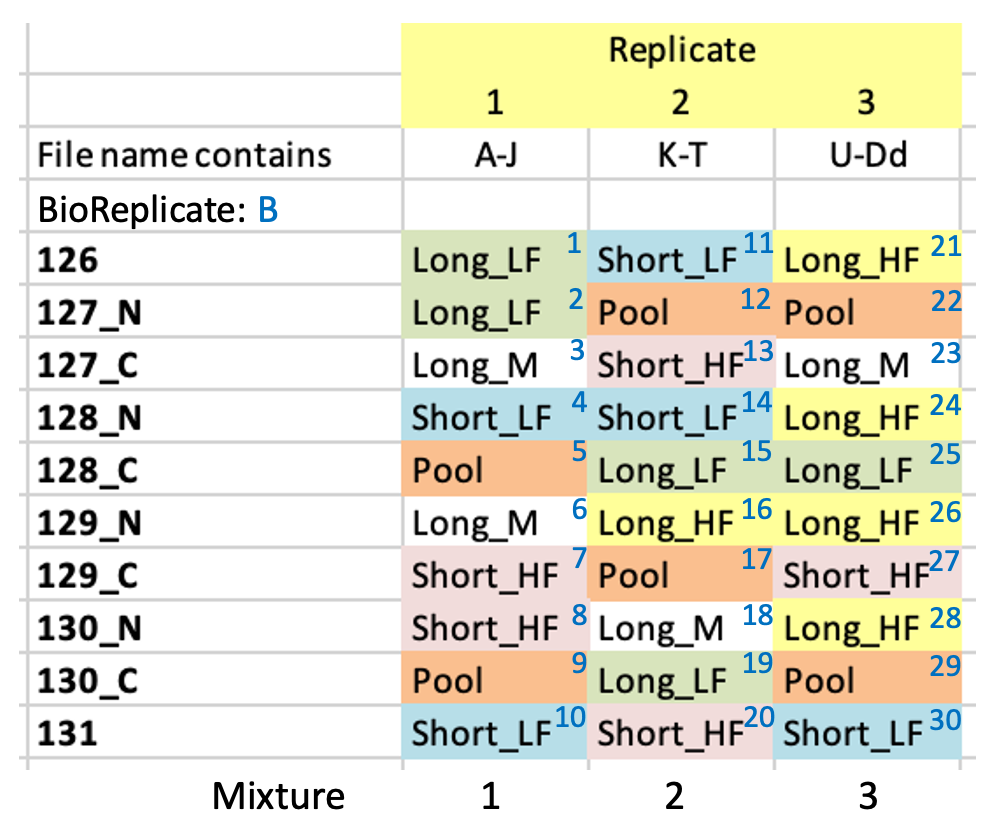
\includegraphics[width=0.95\textwidth]{graphics/isobaric/Dataset_MSstatsTMT.png}
%  \caption{Dataset}
%  \label{fig:isobaric_dataset_plubell}
%\end{figure}
%
%\subsection{Experimental Design (TMT)}
%The experimental design for a TMT experiment is similar to a LFQ experiment. The difference is in the available channels and possible Mixtures. 
%
%\begin{table}[!ht]
%\centering
%\small
%\begin{tabular*}{0.95\textwidth}{lllll}
%Spectra\_Filepath                         & Fraction           & Label                 & Fraction\_Group  & Sample    \\
%PAMI-176\_Mouse\_A-J\_TMT\_14pctACN.mzML  & 1                  & 1                     & 1                & 1         \\
%PAMI-176\_Mouse\_A-J\_TMT\_14pctACN.mzML  & 1                  & 2                     & 1                & 2         \\
%PAMI-176\_Mouse\_A-J\_TMT\_14pctACN.mzML  & 1                  & 3                     & 1                & 3         \\
%PAMI-176\_Mouse\_A-J\_TMT\_14pctACN.mzML  & 1                  & 4                     & 1                & 4         \\
%PAMI-176\_Mouse\_A-J\_TMT\_14pctACN.mzML  & 1                  & 5                     & 1                & 5         \\
%PAMI-176\_Mouse\_A-J\_TMT\_14pctACN.mzML  & 1                  & 6                     & 1                & 6         \\
%PAMI-176\_Mouse\_A-J\_TMT\_14pctACN.mzML  & 1                  & 7                     & 1                & 7         \\
%PAMI-176\_Mouse\_A-J\_TMT\_14pctACN.mzML  & 1                  & 8                     & 1                & 8         \\
%PAMI-176\_Mouse\_A-J\_TMT\_14pctACN.mzML  & 1                  & 9                     & 1                & 9         \\
%PAMI-176\_Mouse\_A-J\_TMT\_14pctACN.mzML  & 1                  & 10                    & 1                & 10        \\
%PAMI-176\_Mouse\_K-T\_TMT\_14pctACN.mzML  & 1                  & 1                     & 2                & 11        \\
%PAMI-176\_Mouse\_K-T\_TMT\_14pctACN.mzML  & 1                  & 2                     & 2                & 12        \\
%PAMI-176\_Mouse\_K-T\_TMT\_14pctACN.mzML  & 1                  & 3                     & 2                & 13        \\
%PAMI-176\_Mouse\_K-T\_TMT\_14pctACN.mzML  & 1                  & 4                     & 2                & 14        \\
%PAMI-176\_Mouse\_K-T\_TMT\_14pctACN.mzML  & 1                  & 5                     & 2                & 15        \\
%PAMI-176\_Mouse\_K-T\_TMT\_14pctACN.mzML  & 1                  & 6                     & 2                & 16        \\
%PAMI-176\_Mouse\_K-T\_TMT\_14pctACN.mzML  & 1                  & 7                     & 2                & 17        \\
%PAMI-176\_Mouse\_K-T\_TMT\_14pctACN.mzML  & 1                  & 8                     & 2                & 18        \\
%PAMI-176\_Mouse\_K-T\_TMT\_14pctACN.mzML  & 1                  & 9                     & 2                & 19        \\
%PAMI-176\_Mouse\_K-T\_TMT\_14pctACN.mzML  & 1                  & 10                    & 2                & 20        \\
%PAMI-194\_Mouse\_U-Dd\_TMT\_14pctACN.mzML & 1                  & 1                     & 3                & 21        \\
%PAMI-194\_Mouse\_U-Dd\_TMT\_14pctACN.mzML & 1                  & 2                     & 3                & 22        \\
%PAMI-194\_Mouse\_U-Dd\_TMT\_14pctACN.mzML & 1                  & 3                     & 3                & 23        \\
%PAMI-194\_Mouse\_U-Dd\_TMT\_14pctACN.mzML & 1                  & 4                     & 3                & 24        \\
%PAMI-194\_Mouse\_U-Dd\_TMT\_14pctACN.mzML & 1                  & 5                     & 3                & 25        \\
%PAMI-194\_Mouse\_U-Dd\_TMT\_14pctACN.mzML & 1                  & 6                     & 3                & 26        \\
%PAMI-194\_Mouse\_U-Dd\_TMT\_14pctACN.mzML & 1                  & 7                     & 3                & 27        \\
%PAMI-194\_Mouse\_U-Dd\_TMT\_14pctACN.mzML & 1                  & 8                     & 3                & 28        \\
%PAMI-194\_Mouse\_U-Dd\_TMT\_14pctACN.mzML & 1                  & 9                     & 3                & 29        \\
%PAMI-194\_Mouse\_U-Dd\_TMT\_14pctACN.mzML & 1                  & 10                    & 3                & 30        \\
%\end{tabular*}
%\end{table}
%
%\begin{table}[!ht]
%\centering
%\small
%\begin{tabular*}{0.95\textwidth}{lllll}
%Sample                                    & MSstats\_Condition & MSstats\_BioReplicate & MSstats\_Mixture & LabelName \\
%1                                         & Long\_LF           & 1                     & 1                & 126       \\
%2                                         & Long\_LF           & 2                     & 1                & 127N      \\
%3                                         & Long\_M            & 3                     & 1                & 127C      \\
%4                                         & Short\_LF          & 4                     & 1                & 128N      \\
%5                                         & Norm               & 5                     & 1                & 128C      \\
%6                                         & Long\_M            & 6                     & 1                & 129N      \\
%7                                         & Short\_HF          & 7                     & 1                & 129C      \\
%8                                         & Short\_HF          & 8                     & 1                & 130N      \\
%9                                         & Norm               & 9                     & 1                & 130C      \\
%10                                        & Short\_LF          & 10                    & 1                & 131       \\
%11                                        & Short\_LF          & 11                    & 2                & 126       \\
%12                                        & Norm               & 12                    & 2                & 127N      \\
%13                                        & Short\_HF          & 13                    & 2                & 127C      \\
%14                                        & Short\_LF          & 14                    & 2                & 128N      \\
%15                                        & Long\_LF           & 15                    & 2                & 128C      \\
%16                                        & Long\_HF           & 16                    & 2                & 129N      \\
%17                                        & Norm               & 17                    & 2                & 129C      \\
%18                                        & Long\_M            & 18                    & 2                & 130N      \\
%19                                        & Long\_LF           & 19                    & 2                & 130C      \\
%20                                        & Short\_HF          & 20                    & 2                & 131       \\
%21                                        & Long\_HF           & 21                    & 3                & 126       \\
%22                                        & Norm               & 22                    & 3                & 127N      \\
%23                                        & Long\_M            & 23                    & 3                & 127C      \\
%24                                        & Long\_HF           & 24                    & 3                & 128N      \\
%25                                        & Long\_LF           & 25                    & 3                & 128C      \\
%26                                        & Long\_HF           & 26                    & 3                & 129N      \\
%27                                        & Short\_HF          & 27                    & 3                & 129C      \\
%28                                        & Long\_HF           & 28                    & 3                & 130N      \\
%29                                        & Norm               & 29                    & 3                & 130C      \\
%30                                        & Short\_LF          & 30                    & 3                & 131      
%\end{tabular*}
%\end{table}
